\documentclass[11pt,a4paper]{article}

\usepackage{etex}
\usepackage[applemac]{inputenc}
\usepackage{latexsym}
\usepackage{graphicx}
\usepackage[francais]{babel}
\usepackage{amsmath,amssymb}
\usepackage{pstricks,pst-plot}
\usepackage{calc}
\usepackage{multicol}
\usepackage{fancyhdr}
\usepackage{lastpage}
\usepackage[T1]{fontenc}
\usepackage{stmaryrd}
\usepackage{float}
\pagestyle{plain}
\usepackage[top=2cm, bottom=2cm, left=3cm, right=3cm]{geometry}

\usepackage{tikz}
\usetikzlibrary{arrows}

\newcommand{\indep}{\rotatebox[origin=c]{90}{$\models$}}

	\title{Probabilistic Graphical Models : Assignment 2}
	\author{Mathurin \textsc{Massias} \and Cl�ment \textsc{Nicolle}}
	\date{\today}

\begin{document}
	
	\maketitle

\section{Distributions factorizing in a graph}

\hspace*{-6mm}\textit{(a)}
\\i. This is a covered edge, for example :
\\
\begin{center}
\begin{tikzpicture}[->,>=stealth',shorten >=1pt,auto,node distance=2cm,
thick,main node/.style={circle,draw,font=\sffamily\Large\bfseries}]

\node[main node] (1) {};
\node[main node] (2) [below of=1] {i};
\node[main node] (3) [right of=2] {j};
\node[main node] (4) [below of=2] {};

\path[every node/.style={font=\sffamily\small}]
	(1) edge node {} (2)
	edge node {} (3)
	(2) edge node {} (3)
	(4) edge node  {} (2)
	edge node {} (3);

\end{tikzpicture}
\end{center}
%
The parents of the node $j$ are $\left\lbrace  i + parents\:of\:i \right\rbrace$. We now reverse $i \rightarrow j$. Let show that $\mathcal{L}(G) = \mathcal{L}(G')$
\\
\\
If $p(x) \in \mathcal{L(G)}$ we have :
\\$p(x) = \mathop{\Pi}\limits_{k=1}^N p(x_k | x_{\pi_k}) = \mathop{\Pi}\limits_{k \not\in \left\lbrace i,j \right\rbrace} p(x_k | x_{\pi_k}) \times p(x_i | x_{\pi_i}) \times p(x_j | x_{\pi_j}) $
\\
But, with $\pi_j = \pi_i \cup \left\lbrace i \right\rbrace$, we have :
\\
$p(x_i | x_{\pi_i}) \times p(x_j | x_{\pi_j}) = p(x_i | x_{\pi_i}) \times p(x_j | x_{\pi_i}, x_i) = p(x_i | x_{\pi_i}) \times p(x_j | x_{\pi_i})$
\\ \-\hspace{1cm} because $x_i$ depends on $x_{\pi_i}$
\\And if we reverse  $i \rightarrow j$, $x_{\pi_i}$ becomes $x_{\pi_j}$ and the value of the product above will be the same.
\\
\\
So $\mathcal{L}(G) = \mathcal{L}(G')$
\\
\\
ii. Let $G$ be a directed tree without v-structures and $G'$ the undirected tree with the same edges (the symmetrized graph). Let show that $\mathcal{L}(G) = \mathcal{L}(G')$
\\
\\
As there is no v-structures in $G$, it means that the cliques of $G'$ are only composed of couples : $C= \left\lbrace (x_i, x_{\pi_i}) \right\rbrace$ (each $x_i$ has a single parent).
\\Thus we have $p(x) = \mathop{\Pi}\limits_{c=1}^N p(x_c | x_{\pi_c}) = \frac{1}{Z} \mathop{\Pi}\limits_{c \in C} \psi_c (x_c) $ with $\psi_c (x_c) \: \alpha \: p(x_c | x_{\pi_c})$
\\
\\
So $\mathcal{L}(G) = \mathcal{L}(G')$
\\
\\
\textit{(b)}
\\According to (a)ii., if the number of nodes is 1 or 2 we have no v-structures so $\mathcal{L}(G) = \mathcal{L}(G')$.
For 3 nodes, we need to oblige to have a v-structure in the directed graph. If we choose an undirected graph where the three nodes ae linked, we will compulsorily have a v-structure, as below :

\begin{center}
\begin{tikzpicture}[->,>=stealth',shorten >=1pt,auto,node distance=2cm,
thick,main node/.style={circle,draw,font=\sffamily\Large\bfseries}]

\node[main node] (1) {1};
\node[main node] (2) [below of=1] {2};
\node[main node] (3) [right of=2] {3};

\path[every node/.style={font=\sffamily\small}]
(1) edge node {} (2)
	edge node {} (3)
(2) edge node {} (3);

\end{tikzpicture}
\end{center}

So the symmetrized graph is composed of only one maximal clique, but we have $p(x) = p(x_1) \times p(x_2 | x_1) \times p(x_3 | x_1, x_2)$, which cannot be written as $\psi(x_1, x_2, x_3)$

\section{d-separation}
%
%
\hspace*{-6mm}\textit{(a)}
\\If $G = (V,E)$, the moralized graph is $G_M = (V,E')$ with $E' = E \cup \left\lbrace (i,j) / \exists k \in V \: s.t. \: i,j \in \pi_k \right\rbrace$
\\Let's take a chain $(v_1,...,v_N)$ from A to B in $G$. It is also a chain in $G_M$. As S separates A and B in $G_M$, we know that this chain goes through S, which means it exists i such that $v_i \in S$.
\\We can consider without loss of generality that this i is unique (if the chain goes through consecutive vertices in S we group them in one, and if it goes through several disjoint vertices we can cut it in different subchains with only one vertice in S).
\\From here, we have two cases :
\\- $(v_{i-1},v_i,v_{i+1})$ is not a v-structure in $G$. Then we have that $v_i \in S$ blocks the chain.
\\- $(v_{i-1},v_i,v_{i+1})$ is a v-structure in $G$.
\\Then $v_{i-1}$ and $v_{i+1}$ are linked in $G_M$ because they are both parent of $v_i$. So the chain $(v_1,...,v_{i-1},v{i+1},...,v_N)$ goes from A to B in $G_M$. Then, this chains goes through S in $G_M$, which is absurd because we made the assumptions that $v_i$ was the unique vertice in S from the chain. \\So $(v_{i-1},v_i,v_{i+1})$ cannot be a v-structure.
\\
\\To sum up, every chains from A to B go through S and there is no v-structure on such vertices. So A and B are d-separated by S in $G$.
\\
\\\textit{(b)}
\\No, this is not true. Here is a counterexample :

\begin{center}
\begin{tikzpicture}[->,>=stealth',shorten >=1pt,auto,node distance=2cm,
thick,main node/.style={circle,draw,font=\sffamily\Large\bfseries}]
	
\node[main node] (1) {};
\node[main node] (2) [below right of=1] {S};
\node[main node] (3) [above right of=1] {A};
\node[main node] (4) [right of=3] {};
\node[main node] (5) [below right of=4] {T};
\node[main node] (6) [above right of=5] {};
\node[main node] (7) [right of=6] {B};
	
\path[every node/.style={font=\sffamily\small}]
(1) edge node {} (2)
edge node {} (3)
(3) edge node {} (4)
(4) edge node {} (5)
(6) edge node {} (5)
edge node {} (7);
	
	\end{tikzpicture}
\end{center}
S separates A and B as the only chain that goes from A to B contains a v-structure on T which is not in S.
\\T separates A and S as the only chain that goes from A to B contains a v-structure on a vertice which is not in T.
\\But T does not separates A and B, because the only chain that goes from A to B contains a v-structure on T.
\\
\\\textit{(c)}
\\ We know that if A and B are d-separated by S, then $X_A \indep X_B | X_C$.
\\- $X_{\left\lbrace 1,2 \right\rbrace} \indep X_4 | X_3$ : True.
\\3 separates $\left\lbrace 1,2 \right\rbrace$ and 4 because the chains from $\left\lbrace 1,2 \right\rbrace$ to 4 have a v-structure on 8 which is not an ancestor of 3.
\\
\\- $X_{\left\lbrace 1,2 \right\rbrace} \indep X_4 | X_5$ : False, because 5 is a descendant of 8 where we have a v-structure.
\\
\\$X_1 \indep X_6 | X_{\left\lbrace 2,4,7 \right\rbrace}$ : True
\\All chain from 1 to 6 go through 7 with no v-structure.

\section{Implementation of K Means and Gaussian mixture}
%
%
\textit{(a)}
Running our algorithm with a different seed each time, we see that it can converge to different results, some of them quite bad (seed=44 gives a distorsion of 1500, whereas usually distorsion is around 1100).
\begin{figure}[H]
\centering
\noindent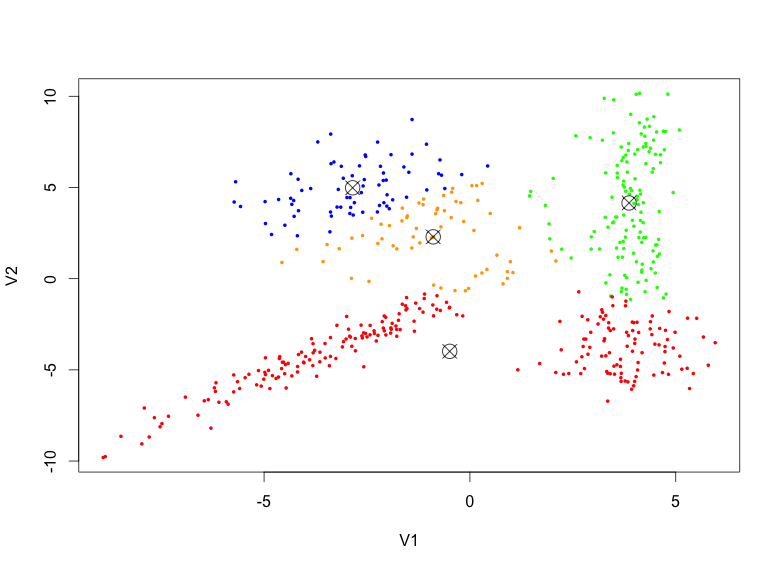
\includegraphics[scale=0.5]{kmeans_pourri.png}
\noindent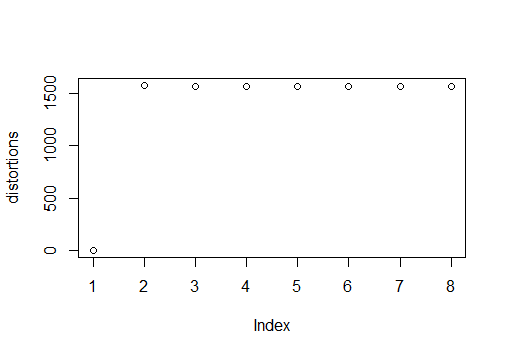
\includegraphics[scale=0.5]{distortion_seed44.png}
\caption{Clusters and centroids obtained by K-Means for seed = 44, and distortion measure at each iteration (starting arbitrarily to 0)}
\end{figure}

\begin{figure}[H]
\centering
\noindent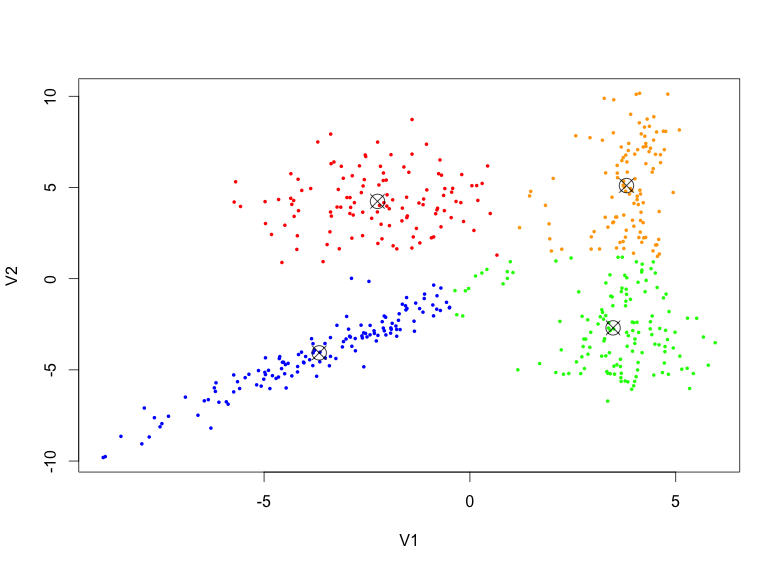
\includegraphics[scale=0.5]{kmeans_good.png}
\noindent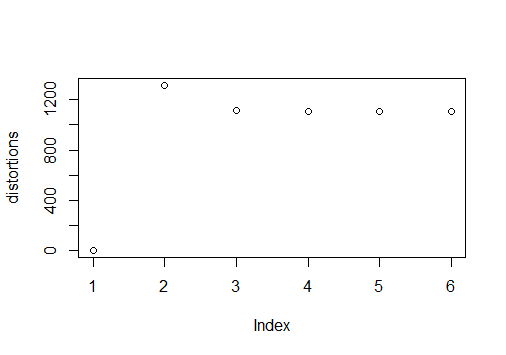
\includegraphics[scale=0.5]{distortion_seed45.png}
\caption{Clusters and centroids obtained by K-Means for seed = 45, and distortion measure at each iteration (starting arbitrarily to 0)}
\end{figure}

\textit{(b)}
\begin{figure}[H]
\centering
\noindent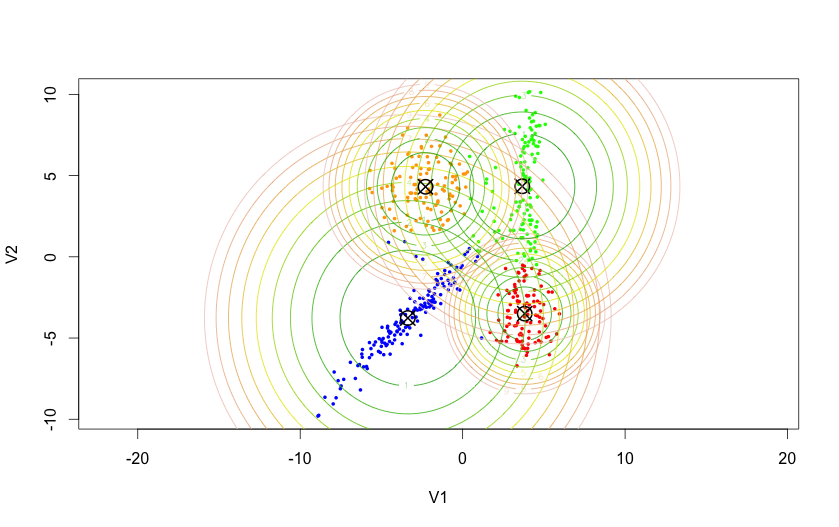
\includegraphics[scale=0.5]{circles.png}
\caption{Data set and 4 gaussians with their level sets (circles), from 10\% to 90\%}
\end{figure}
As we forced the variances to be proportional to $I_2$, we get that level sets are circles, because we have $(x-\mu)^T \Sigma^{-1} (x- \mu) = \frac{1}{\sigma^2} \Vert x - \mu \Vert ^2$.
%
%
\\[5mm]\textit{(c)}
\begin{figure}[H]
\centering
\noindent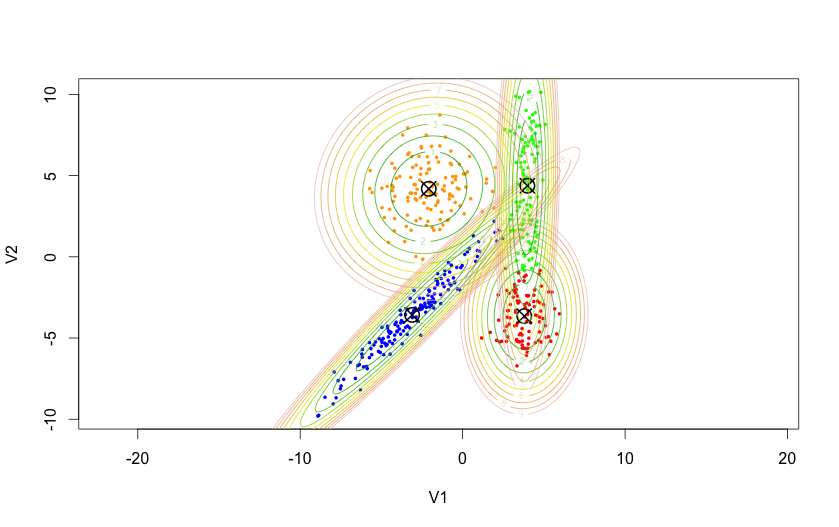
\includegraphics[scale=0.5]{ellipsis.png}
\caption{Data set and 4 gaussians with their level sets (ellipsis), from 10\% to 90\%}
\end{figure}
Since no assumption is made on the 4 variances, the level sets are now ellipsis, whose axis are not necessarily parallel to $(Ox)$ and $(Oy)$ respectively. Had we imposed that the variances should be diagonal, we would have obtained ellipsis with such axis.
%
%TODO question d
\\[5mm]
\textit{(d)} 
When we impose the variances to be diagonal, on the training set we get a final log-likelihood of approx - 2700. When we relax this constraint, we get a final llh  of approx -2350 : relaxing constrains allows the model to better fit the data.
\\
\\
On test data, we obtain a log-likelihood of approx -2650 with the Gaussian Mixtures model trained with diagonal variances. As the test dataset has the same size as the training one, we see here that the test dataset better fits to the model that the train set itself. 
\\With the general Gaussian Mixtures model trained (no assumption made on covariance matrix), we obtain a llh of approx -2420. It is in the same range than for train data.
\end{document}